Since the beginning of data collection, an important question we try to answer is how do we define a semantic unit in the sketch?  
The end goal is to achieve the kind of interaction shown in the YouTube video \textit{How To Draw A Cute Ice Cream Cone}, and in it, the instructor oftens uses sentences in the form of ``Let's draw a \texttt{X} for the \texttt{Y}'', where \texttt{X} describes the geometric features of the object \texttt{Y}. For example, ``Let's draw \textit{small connected U shapes} for the \textit{bottom of the ice-cream cone}.'' Therefore, at first, we thought of decomposing the drawing process into a sequence of common geometric shapes, and the objects that they represent become the basic semantic units.      
asdfasd sdfdsfsd
Version 0 was never deployed. I think at this stage of the data collection, we are trying to decide whether there should be a fixed set of primitive that the users could choose from, so learning the model becomes learning to parameterize, for example, the dimensions of the set of primitives. 

Functionality:
\begin{itemize}
    \item Draw the figure and the page will record the sequence 
    \item User can replay its drawing sequence. The original idea was that users will first create the drawing, and then they can replay the sequence as they annotate for each step. 
\end{itemize}

The very first test version:
In terms of the main task, I created a test version to confirm that the idea of the drawing board is sensible.

Press \textit{Record}, Draw on the board, Press \textit{Stop} when done with drawing, \textit{Submit} the drawing if one is satisfied with the quality, \textit{Play} to revisit the drawing, \textit{Cancel} to start over. 

What was the original motivation behind this functionality was that it will aid the annotators to review the drawing process and divide it into better steps. Responding to DQ \ref{data_design_1}. 
However, in this very crude version, we did not really incorporate features for either 
Responding to DQ \ref{data_design_2}, 

We begin with a very crude version, and then we decide to add features that can allow us to realize the DQ \ref{data_design_1} and \ref{data_design_2}.

The actual Version 0 has the following flow:
There is a practice board, you can try to practice drawing so that the actual drawing submit has good quality and respond to the prompt (reflecting DQ \ref{data_design_3}). Then hit \textit{Ready to Record}, again baking the sequence into the design of the website will help us to enforce collecting a dataset of steps. Another purpose is to help the annotators decide beforehand what are the necessary primitives used in the process. Why was I so fixated on the primitives, because the abstractness of the icons is what interested me the most. The entire research journey was very explorative, it sorted of started with a sense of \textit{oh, this question or aspect of how humans do things is interesting, I wish robot can do the same}. And what is that thing that I thought was interesting, it was how Rain and I were able to draw the icons and the interactions. 
The first thing you will do is select a primitive from a list, and then you will draw the step that contains the primitives. Hit \textit{Next} to move on to drawing the next primitive. There are will be a little tag at the bottom showing what is the primitive that corresponds to the step that is drawn on the board. Repeat until finished and hit \textit{Done}. At the end, again, \textit{Play}, \textit{Submit}, or \textit{Cancel} to start over. 

{\color{red} \faIcon{question}} Should we use primitive shapes for users to choose from? 
The reason for considering this aspect is whether during generation we want to learn to change parameters of a fix set of shapes or generate un-constrained strokes. For the first option, we want users to compose a drawing with primitive shapes, much like using   
In order to learn a more general model, we decided that we want to collect strokes instead of fixed primitive shapes, so we moved onto creating a table that accompanies the drawing board, where the user can choose to annotate each step they draw. We can see in Figure \ref{v0.design}.

\begin{figure*}[h!]
\begin{subfigure}{\textwidth}
  \centering
  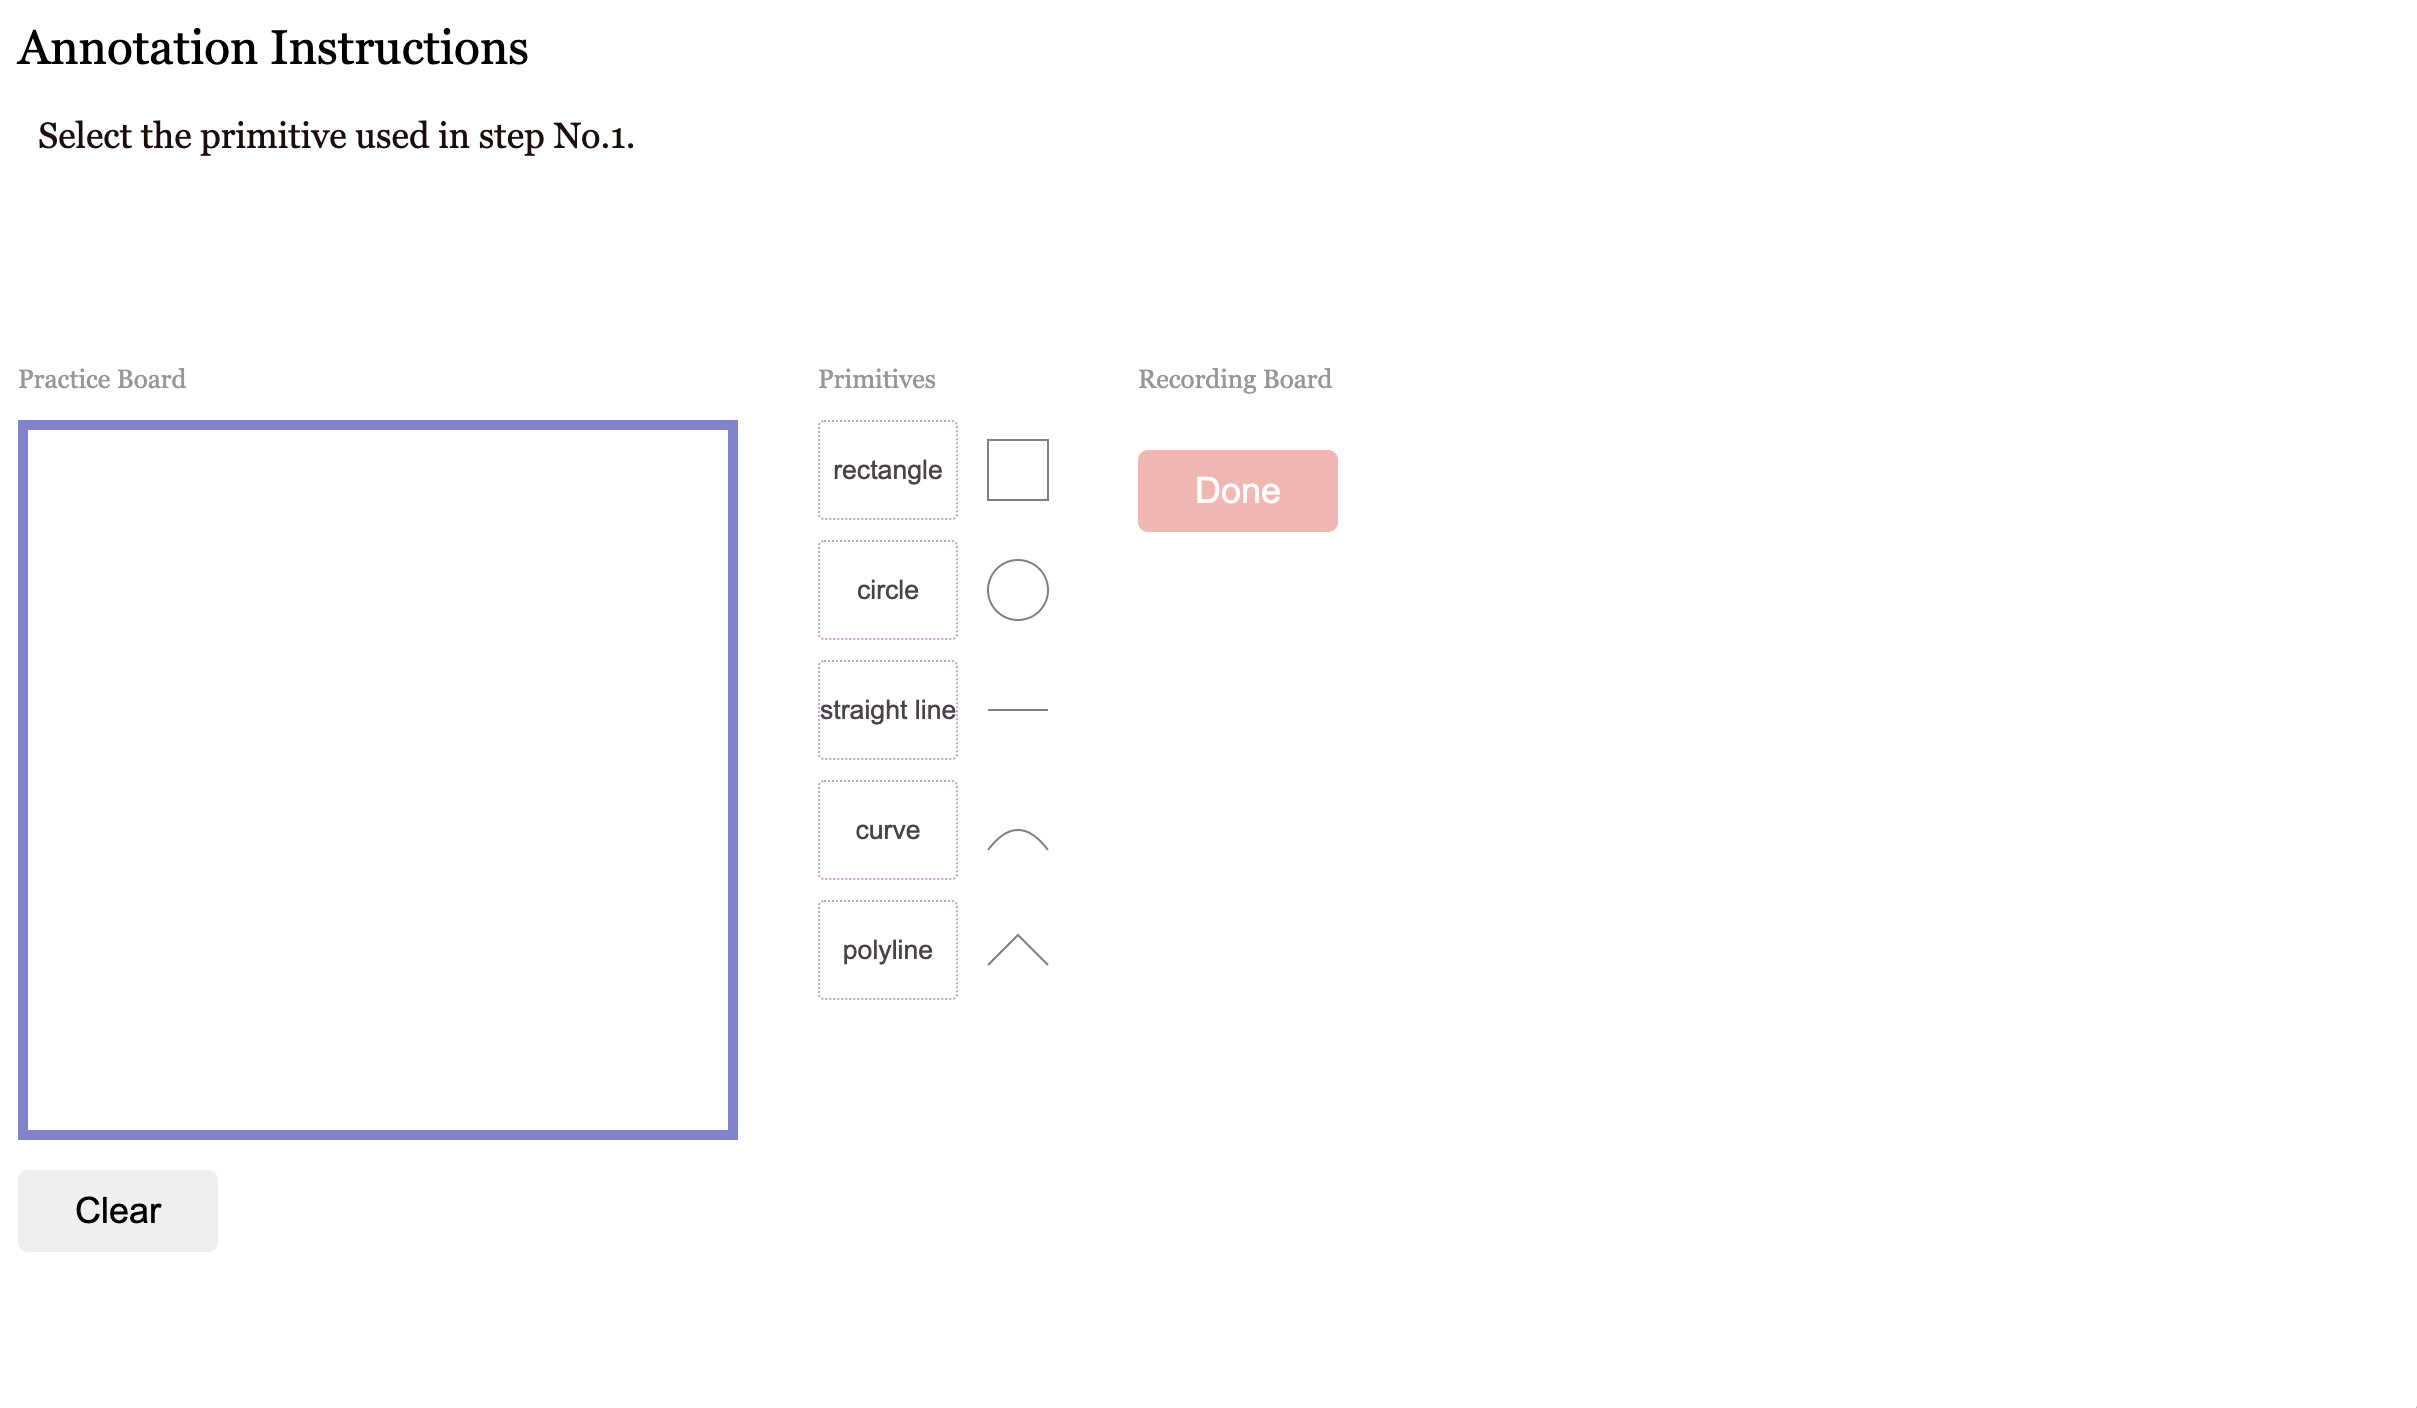
\includegraphics[width=.8\linewidth]{data_collection/version_0_select_primitive.png}
  \caption{Design of main task for third pilot.}
  \label{v0.1}
\end{subfigure}
\newline
\begin{subfigure}{\textwidth}
  \centering
  % include third image
  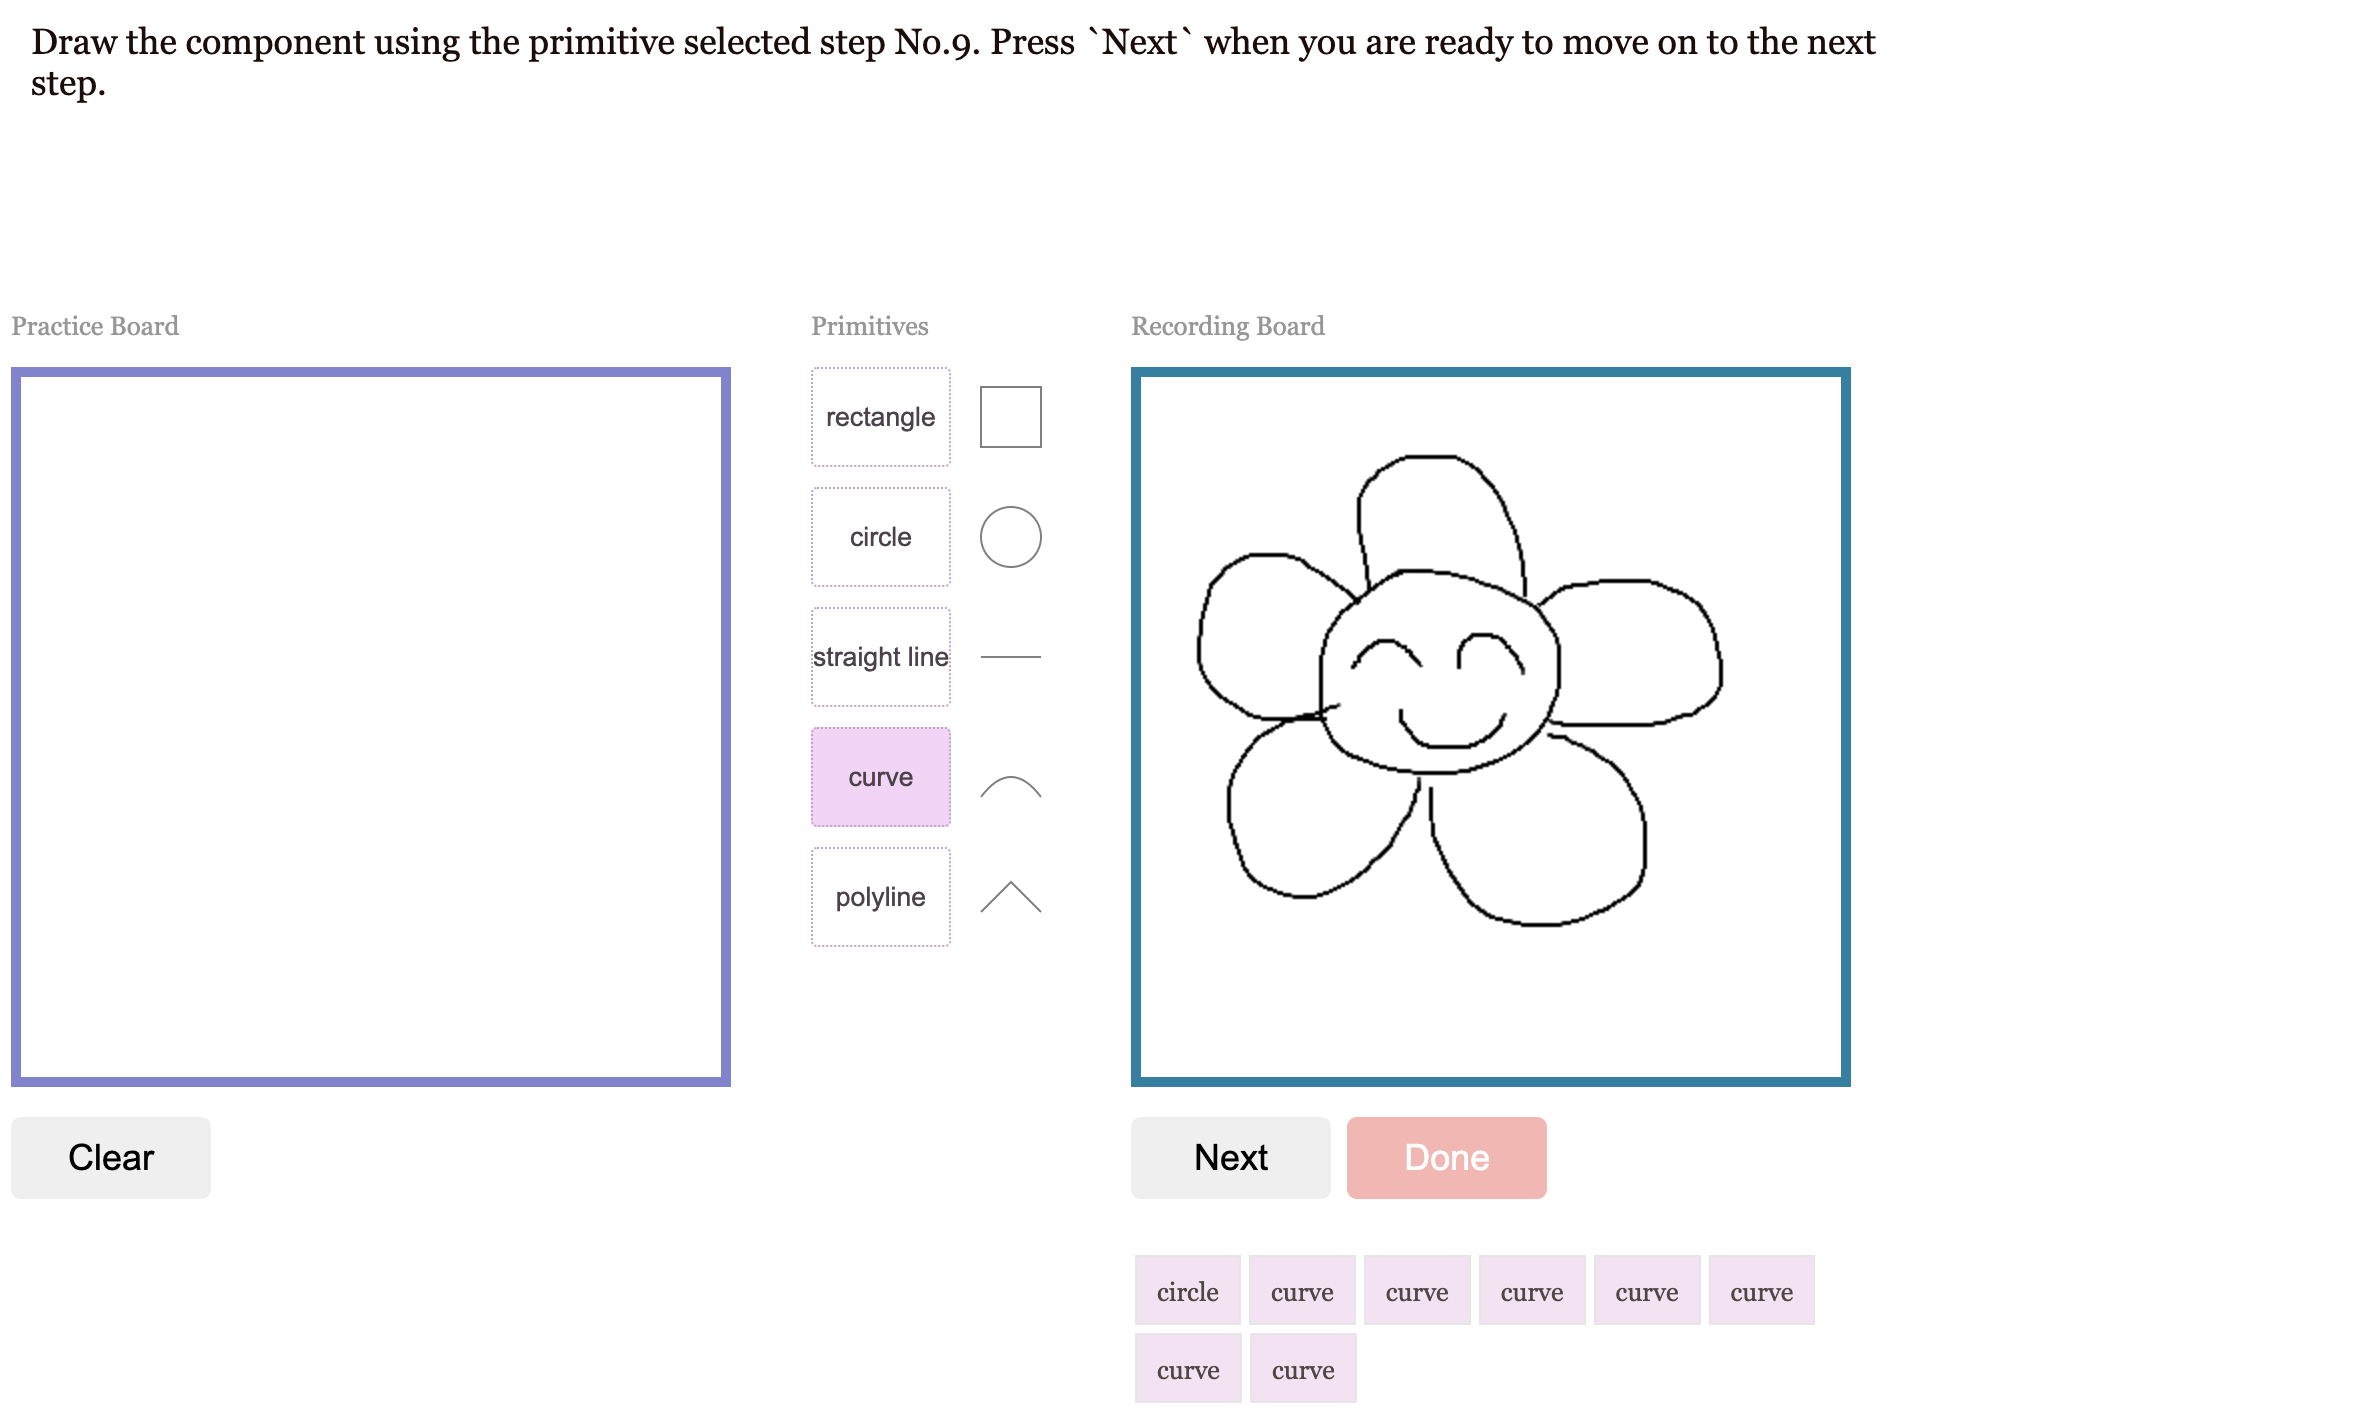
\includegraphics[width=.8\linewidth]{data_collection/version_0_smiley_flower_with_primitive.png}  
  \caption{Design of main task for final task.}
  \label{v0.1}
\end{subfigure}
\caption{Progress of the design two for the main task in version two.}
\label{v0.design}
\end{figure*}